% questions.tex —— 1977 年·山东A卷 · 题目内容片段（无答案）
% 由 tools/generate_projects.py 依来源总账自 1977/1977_数学真题_山东A_试题.md 生成，勿手改（改源 MD 后重跑）


\gkpart{数学试题解（山东A卷）}

\begin{gktip}
\textbf{来源说明}：本题面依据固定源 PDF《山东1977年高考数学试题解》第 1—5 页逐题转录。源卷为题面与解答连续排印的扫描材料（书籍页码 51—54，末页无页码），解答部分供答案要点与解析正文对照复算之用。正式题为第一大题（含 6 个小题，每小题 5 分）与第二至第六大题共 6 道；卷末另有「参考题」2 道，注明不作录取成绩，不计入题量。原卷无文理科目说明。源卷函数记号 Cos、Sin、Lg、Log、Lim 按现代通行写法转写为 cos、sin、lg、log、lim。
\end{gktip}

\Needspace{0.4\textheight}
\begin{question}
\gkti{1}解下列各题（每小题 5 分）：

（1） $\sqrt{(3-x)^2}=?$

（2） $\lg 2+\lg 5+\lg\sqrt{10}+\lg 0.01+\log_8\log_3 3=?$

（3） 写出函数定义域：

① $y=\log_a x$（$a>0$）；

② $y=\dfrac{\sqrt{x-1}}{x+3}$。

（4） 写出过点 $(2,3)$ 斜率为 $-\dfrac12$ 的直线方程。

（5） 求椭园 $\dfrac{x^2}{25}+\dfrac{y^2}{16}=1$ 的焦点坐标。

\begin{gktip}
\textbf{源注}：原卷印作「椭园」，系「椭圆」之排印变体，本文保留原文字形。
\end{gktip}

（6） 如右图所示的三视图是什么几何体？
\nopagebreak[4]
\begin{center}% 1977 年山东A卷第 1（6）题：正四棱台的三视图——上排为正视图、左视图（两个等腰梯形，带点划线对称轴），下排为俯视图（外大内小两个正方形、四角相连）（按源卷第 2 页布局）
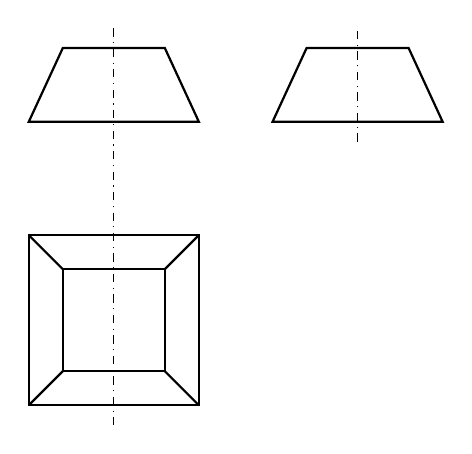
\begin{tikzpicture}[scale=0.72]
  % 正视图（左上）
  \draw[thick] (-1.5,0) -- (1.5,0) -- (0.9,1.3) -- (-0.9,1.3) -- cycle;
  \draw[dashdotted] (0,1.65) -- (0,-5.35);
  % 左视图（右上）
  \begin{scope}[shift={(4.3,0)}]
    \draw[thick] (-1.5,0) -- (1.5,0) -- (0.9,1.3) -- (-0.9,1.3) -- cycle;
    \draw[dashdotted] (0,-0.35) -- (0,1.65);
  \end{scope}
  % 俯视图（左下）
  \draw[thick] (-1.5,-5.0) rectangle (1.5,-2.0);
  \draw[thick] (-0.9,-4.4) rectangle (0.9,-2.6);
  \draw[thick] (-1.5,-2.0) -- (-0.9,-2.6);
  \draw[thick] (1.5,-2.0) -- (0.9,-2.6);
  \draw[thick] (-1.5,-5.0) -- (-0.9,-4.4);
  \draw[thick] (1.5,-5.0) -- (0.9,-4.4);
\end{tikzpicture}
\end{center}
\nopagebreak[4]
\Needspace{0.4\textheight}
\end{question}
\begin{question}
\gkti{2}\textbf{（10 分）} 设 $AD$ 是 $\triangle ABC$ 的高，在线段 $BC$ 上取点 $E$，使 $\angle EAC=\angle BAD$，延长 $AE$ 交 $\triangle ABC$ 外接圆于点 $F$。求证：$AF$ 是外接圆的直径。
\nopagebreak[4]
\begin{center}% 1977 年山东A卷第 2 题：三角形 ABC 的外接圆，AD 为高（D 在 BC 上），E 在 BC 上且 A、E、F 共线，F 为 AE 延长线与圆的交点，CF 为虚线辅助线（按源卷第 2 页布局）
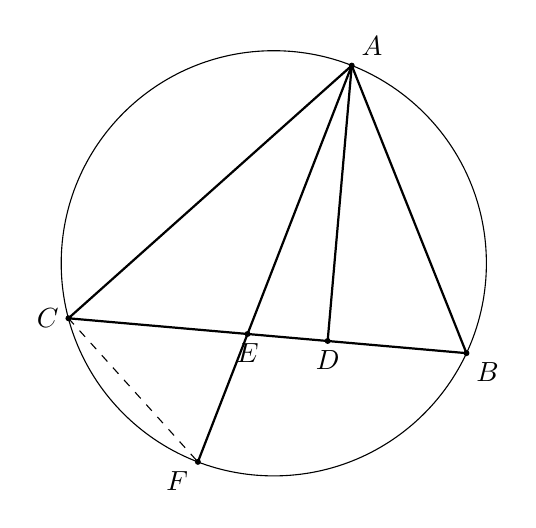
\begin{tikzpicture}[scale=0.9]
  \draw (0,0) circle (3);
  \coordinate (A) at (1.1,2.79);
  \coordinate (B) at (2.719,-1.268);
  \coordinate (C) at (-2.898,-0.776);
  \coordinate (D) at (0.760,-1.096);
  \coordinate (E) at (-0.370,-0.997);
  \coordinate (F) at (-1.071,-2.802);
  \draw[thick] (A) -- (B) -- (C) -- cycle;
  \draw[thick] (A) -- (D);
  \draw[thick] (A) -- (F);
  \draw[dashed] (C) -- (F);
  \fill (A) circle (1.2pt) node[above right] {$A$};
  \fill (B) circle (1.2pt) node[below right] {$B$};
  \fill (C) circle (1.2pt) node[left] {$C$};
  \fill (D) circle (1.2pt) node[below] {$D$};
  \fill (E) circle (1.2pt) node[below] {$E$};
  \fill (F) circle (1.2pt) node[below left] {$F$};
\end{tikzpicture}
\end{center}
\nopagebreak[4]
\end{question}
\begin{question}
\gkti{3}\textbf{（15 分）} $x^2-x\cos\alpha+\dfrac14\sin^2\alpha=0$（$0<\alpha<\dfrac{\pi}{2}$）为关于 $x$ 的二次方程，当 $\alpha$ 为何值时，方程有两个不相等的实数根？它的根是什么？

\end{question}
\begin{question}
\gkti{4}\textbf{（15 分）} 在半径为 $R$ 的一块圆形铁板上，剪去一个圆心角为 $\alpha$ 弧度的扇形，用剩下的铁板做一个圆锥形容器（铁板厚度和加工量不计）。

（1） 用 $R$ 和 $\alpha$ 表示圆锥底面半径 $r$、圆锥高 $h$、圆锥容积 $V$；

（2） 当 $R=20\,\mathrm{cm}$，$\alpha=\dfrac{2\pi}{5}$ 弧度时，计算圆锥容积 $V$（取 $\pi=3.14$，精确到 $1\,\mathrm{cm^3}$）。

\Needspace{0.4\textheight}
\end{question}
\begin{question}
\gkti{5}\textbf{（15 分）} 我炮兵阵地位于 $A$，两观察所分别设于 $C$、$D$，已知 $\triangle ACD$ 为一正三角形，且 $CD=a$，当目标出现于 $B$ 时，测得 $\angle CDB=45^\circ$，$\angle BCD=75^\circ$，求炮目距离 $AB$。
\nopagebreak[4]
\begin{center}% 1977 年山东A卷第 5 题：△ACD 为正三角形（CD=a，D 左 C 右），A 为炮兵阵地，B 为目标，四点连成带双对角线的四边形（按源卷第 3 页布局）
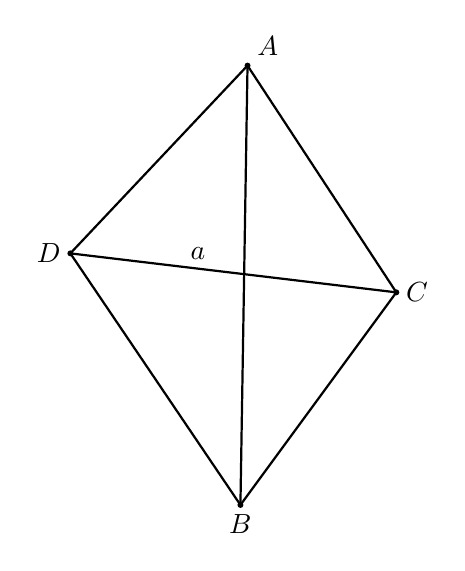
\begin{tikzpicture}[scale=0.9]
  \coordinate (A) at (0.2,3.2);
  \coordinate (D) at (-2.3,0.55);
  \coordinate (C) at (2.3,0);
  \coordinate (B) at (0.1,-3.0);
  \draw[thick] (A) -- (D) -- (C) -- cycle;
  \draw[thick] (A) -- (B);
  \draw[thick] (D) -- (B);
  \draw[thick] (C) -- (B);
  \fill (A) circle (1.2pt) node[above right] {$A$};
  \fill (D) circle (1.2pt) node[left] {$D$};
  \fill (C) circle (1.2pt) node[right] {$C$};
  \fill (B) circle (1.2pt) node[below] {$B$};
  \node at (-0.5,0.55) {$a$};
\end{tikzpicture}
\end{center}
\nopagebreak[4]
\Needspace{0.4\textheight}
\end{question}
\begin{question}
\gkti{6}\textbf{（15 分）} 现有可建猪圈 $L$ 米的材料，要建彼此相连的 $m$ 间面积相等的矩形猪圈（如下图）（门在内，墙的厚度不计）。怎样设计每间猪圈的长和宽，才能使所建的猪圈的总面积最大？按这种设计，$m$ 间猪圈长的总和与宽的总和有什么关系？
\nopagebreak[4]
\begin{center}% 1977 年山东A卷第 6 题：m 间彼此相连的矩形猪圈——整排总长 x 标在上方，每间宽 (L-2x)/(m+1) 标在右侧，下方横线与「m 间」表示整排共 m 间（按源卷第 4 页布局）
\begin{tikzpicture}[scale=0.85]
  \draw[thick] (0,0) rectangle (8,2.4);
  \draw[thick] (1.0,0) -- (1.0,2.4);
  \draw[thick] (2.0,0) -- (2.0,2.4);
  \draw[thick] (3.0,0) -- (3.0,2.4);
  \draw[thick] (4.0,0) -- (4.0,2.4);
  \draw[thick] (6.8,0) -- (6.8,2.4);
  \node at (5.4,1.2) {$\cdots$};
  \node[above] at (4.0,2.55) {$x$};
  \node[right] at (8.2,1.2) {$\dfrac{L-2x}{m+1}$};
  \draw[thick] (0,-0.55) -- (8,-0.55);
  \draw[thick] (0,-0.38) -- (0,-0.72);
  \draw[thick] (8,-0.38) -- (8,-0.72);
  \node[below] at (4.0,-0.78) {$m$ 间};
\end{tikzpicture}
\end{center}
\nopagebreak[4]
\begin{gktip}
\textbf{参考题}（不作录取成绩，考生可视能力尽量作）
\end{gktip}

\Needspace{5\baselineskip}
\textbf{参考题 1．} 求极限：

\nopagebreak[4]
\[
\lim_{x\to\infty}\frac{\mathrm e^x}{x^2}.
\]

\textbf{参考题 2．} 利用定积分证明：椭圆 $\dfrac{x^2}{a^2}+\dfrac{y^2}{b^2}=1$ 的面积 $S=\pi ab$。

\end{question}